\chapter{General Project Context}
\label{chap:General Project Context}

% "*" makes the section unnumbered

\section*{Introduction}

Use this template as you wish, change what you want to change, the section titles are only examples, you don't have to follow them to the letter.


This is an example of me citing the 1st reference in the bibliography at the end of this report \cite{ref1}. Use it well!

The next section contains the README text that's also found in the left part along with the other files.


\newpage

\section{READ\_ME}

Hi! 

This template is a combination of multiple student and teacher PFE report templates that I have compiled into one that hopefully will satisfy your needs.
\\

It is in English, but I have included the french "Page de garde" if you want to use it, and the rest of the paper is easily translatable.
\\

This document is compiled using pdfLatex Compiler, so make sure you select it in the menu on the top left of the page. You can change the font size there along with other things.
\\

Some table, figure, list or formatting codes can be found in the "Codes\_needed.tex" file in this same folder, use them well.
\\

The organisation of this template is as follows: 
\\
The main compilation file is main.tex, any file you want to add, should be added there using, %\chapter{General Project Context}
\label{chap:General Project Context}

% "*" makes the section unnumbered

\section*{Introduction}

Use this template as you wish, change what you want to change, the section titles are only examples, you don't have to follow them to the letter.


This is an example of me citing the 1st reference in the bibliography at the end of this report \cite{ref1}. Use it well!

The next section contains the README text that's also found in the left part along with the other files.


\newpage

\section{READ\_ME}

Hi! 

This template is a combination of multiple student and teacher PFE report templates that I have compiled into one that hopefully will satisfy your needs.
\\

It is in English, but I have included the french "Page de garde" if you want to use it, and the rest of the paper is easily translatable.
\\

This document is compiled using pdfLatex Compiler, so make sure you select it in the menu on the top left of the page. You can change the font size there along with other things.
\\

Some table, figure, list or formatting codes can be found in the "Codes\_needed.tex" file in this same folder, use them well.
\\

The organisation of this template is as follows: 
\\
The main compilation file is main.tex, any file you want to add, should be added there using, %\chapter{General Project Context}
\label{chap:General Project Context}

% "*" makes the section unnumbered

\section*{Introduction}

Use this template as you wish, change what you want to change, the section titles are only examples, you don't have to follow them to the letter.


This is an example of me citing the 1st reference in the bibliography at the end of this report \cite{ref1}. Use it well!

The next section contains the README text that's also found in the left part along with the other files.


\newpage

\section{READ\_ME}

Hi! 

This template is a combination of multiple student and teacher PFE report templates that I have compiled into one that hopefully will satisfy your needs.
\\

It is in English, but I have included the french "Page de garde" if you want to use it, and the rest of the paper is easily translatable.
\\

This document is compiled using pdfLatex Compiler, so make sure you select it in the menu on the top left of the page. You can change the font size there along with other things.
\\

Some table, figure, list or formatting codes can be found in the "Codes\_needed.tex" file in this same folder, use them well.
\\

The organisation of this template is as follows: 
\\
The main compilation file is main.tex, any file you want to add, should be added there using, %\chapter{General Project Context}
\label{chap:General Project Context}

% "*" makes the section unnumbered

\section*{Introduction}

Use this template as you wish, change what you want to change, the section titles are only examples, you don't have to follow them to the letter.


This is an example of me citing the 1st reference in the bibliography at the end of this report \cite{ref1}. Use it well!

The next section contains the README text that's also found in the left part along with the other files.


\newpage

\section{READ\_ME}

Hi! 

This template is a combination of multiple student and teacher PFE report templates that I have compiled into one that hopefully will satisfy your needs.
\\

It is in English, but I have included the french "Page de garde" if you want to use it, and the rest of the paper is easily translatable.
\\

This document is compiled using pdfLatex Compiler, so make sure you select it in the menu on the top left of the page. You can change the font size there along with other things.
\\

Some table, figure, list or formatting codes can be found in the "Codes\_needed.tex" file in this same folder, use them well.
\\

The organisation of this template is as follows: 
\\
The main compilation file is main.tex, any file you want to add, should be added there using, %\input{Chapters/Chapter1} for example. 

Remember to change the PDF Title and author name before the begin document command.
\\

Packages.tex is where you import packages and could modify their options.
\\

The frontmatter folder contains unnumbered chapters that come before the actual chapters, so the resumes and acknowledgments are there. The pages are numbered in Roman numbers.
\\

The chapters folder obviously contains the main chapters of the report, usually the first one is an intro, of both the project and the company, the last one is a conclusion chapter, I made it unnumbered here but you do you.
\\

The endmatter folder contains the appendices, acronyms, glossary, and Complementary figures, tables and codes. Consider checking this link \url{https://libguides.usc.edu/writingguide/appendices} for more info. Usually you add an appendix for each subject you'll talk about it, each with its own codes, tables, figures and text.
\\

The bibliography can be found at the end of main.tex file.
\\

And to organise your figures better, upload the logos to the logos folder, and content related figures should go in the figures folder, where you can add sub folders.
\\

Along the template, make sure to read my comments, they can be helpful to understand the purpose of a command or option. 
\\

When you finish writing your thesis, make sure to verify that you didn't leave any generic line or link. Revise it well.
\\

There are 10 warnings that show up in this template, some I couldn't manage to solve (or understand), and some I left since they are necessary for what I intend of this template.
\\

Obviously this template is only a suggestion, it is not perfect in any sense, you can improve it in the way that suits you, so search away, and get used to reading the documentation.
\\

Also consult with your supervisor, as each teacher has their own opinion on what constitutes the ideal report.
\\

Finally, I hope you have enjoyed your time at INPT as much as I did, and Good Luck :D
\\

-Mery


\subsection{Codes\_Needed}

This subsection includes codes for different elements you will need: figures, tables, lists...

Copy the codes you want and test them in the chapter files.

if you want symbols and other text styles, visit this link: 

\href{https://www.cmor-faculty.rice.edu/~heinken/latex/symbols.pdf}{Symbols}

Read the comments !!

% Content division

%\chapter{Comes first}, then \section{}, then \subsection{}, then \subsubsection{}.

\subsubsection{Text formatting}

\textbf{This text is bold}

\textit{This text is italic}

\underline{This text is underlined.}

\st{This text is struck out.}

\textsc{This text is capitalized.}

%Use \paragraph{To start a paragraph}


Some characters like "\%", "\$" and "\&" are significant in Latex code, so to include them in normal text, use the backslash character before them.
To print out backslash, use \symbol{92}


Documentation: \href{https://www.overleaf.com/learn/latex/Bold%2C_italics_and_underlining}{Italics and underlining}


\subsubsection{Figures} 

\begin{figure}[H] 
    \centering
    
\includegraphics[width=4cm]{Logos/Logo_INPT.png}
    \caption{Caption}
    \label{fig:my_label} %Optional (If you want to reference the figure in later chapters)
\end{figure}

%[width=7cm] you control the size of the image. other options include: 
%[height=7cm] or [scale=0.5] (means half the size of the original image)


Documentation: \href{https://www.overleaf.com/learn/latex/Inserting_Images}{Images}


\subsubsection{Tables} 

Simple table without borders:
\\

\begin{tabular}{ll}
  First & Second \\
  Third & Fourth
\end{tabular}
\\

More complex table with borders:
\\

\begin{tabular}{|l|c|r|} \hline
  Left aligned column & Centered column & Right aligned column \\ \hline
  Text & Text & Text \\ \hline
\end{tabular}
\\

Example of a short table

%{5cm} is the cell length, you can change it to suit your own table

\begin{table}[H]
    \centering
    \begin{tabular}{|m{5cm}|m{10cm}|}
        \hline
          Column1 & Column2 \\
        \hline
          Element11 & Element21 \\
        \hline
          Element12 & Element22 \\
        \hline
          Element13 & Element23 \\
        \hline
    \end{tabular}
    \caption{Table Example}
\end{table}


Example of a long table (that spans 2 pages or more), Latex will automatically split the table when it reaches the end of the page:

\begin{longtable}[c]{| m{4.4cm} | m{11cm} |}
\caption{Long table}\\
 \hline

 Cell & Description  \\ 
 \hline
 \endfirsthead

 \hline
 
 Cell & Description  \\ 
 \hline
 \endhead

        \hline
          Element11 & Element21 \\
        \hline
          Element12 & Element22 \\
        \hline
          Element13 & Element23 \\
        \hline
          Element14 & Element24 \\
        \hline
          Element15 & Element25 \\
        \hline
          Element16 & Element26 \\
        \hline
          Element17 & Element27 \\
        \hline
          Element18 & Element28 \\
        \hline
          Element19 & Element29 \\
        \hline
          Element110 & Element210 \\
        \hline
          Element111 & Element211 \\
        \hline
          Element112 & Element212 \\
        \hline
          Element113 & Element213 \\
        \hline
          Element114 & Element214 \\
        \hline

 \end{longtable}


Documentation: \href{https://www.overleaf.com/learn/latex/Tables}{Tables}


\subsubsection{Lists}

To start an unnumbered list, use:

\begin{itemize}
    \item 
    \item 
    \item 
\end{itemize}

To start a numbered list, use:

\begin{enumerate}
    \item 
    \item 
    \item 
\end{enumerate}



Documentation: \href{https://www.overleaf.com/learn/latex/Lists}{Lists}


\subsubsection{Code scripts or terminal}

Say you have a script or terminal command you want to include, you use the following code:

    \lstset{style=mystyle} %this style is already defined in Packages.tex
    
    \begin{lstlisting}[language=bash, caption= Code caption]
    
    root@eve-ng:~# mkdir -p /opt/unetlab/addons/qemu/timos-20.10.R12

    \end{lstlisting}


Documentation: \href{https://www.overleaf.com/learn/latex/Code_listing}{Code Listing}

\subsubsection{Math}

Some math formulas for you, test them in your chapters:

These are inline formulas: $x$, $a_i^2 + b_i^2 \le a_{i+1}^2$. Afterwards...

These are centered formulas: $$x,$$ $$a_i^2 + b_i^2 \le a_{i+1}^2.$$ Afterwards...

Some complex formula: $$P(|S - E[S]| \ge t) \le 2 \exp \left( -\frac{2 t^2 n^2}{\sum_{i = 1}^n (b_i - a_i)^2} \right).$$

Also you can use the first link for math symbols and other useful stuff:

Documentation: \href{https://www.cmor-faculty.rice.edu/~heinken/latex/symbols.pdf}{Symbols file again}



\newpage


\section{Presentation of host organization}



\subsection{Company Overview}

\begin{figure}[H] 
    \centering
    \includegraphics[width=7cm]{Logos/Company_Logo_Expl.png}
    \caption{Company logo}
    %\label{fig:my_label} %Optional (If you want to reference the figure in later chapters)
\end{figure}



\subsection{Organizational Chart}


\begin{figure}[H] 
    \centering
    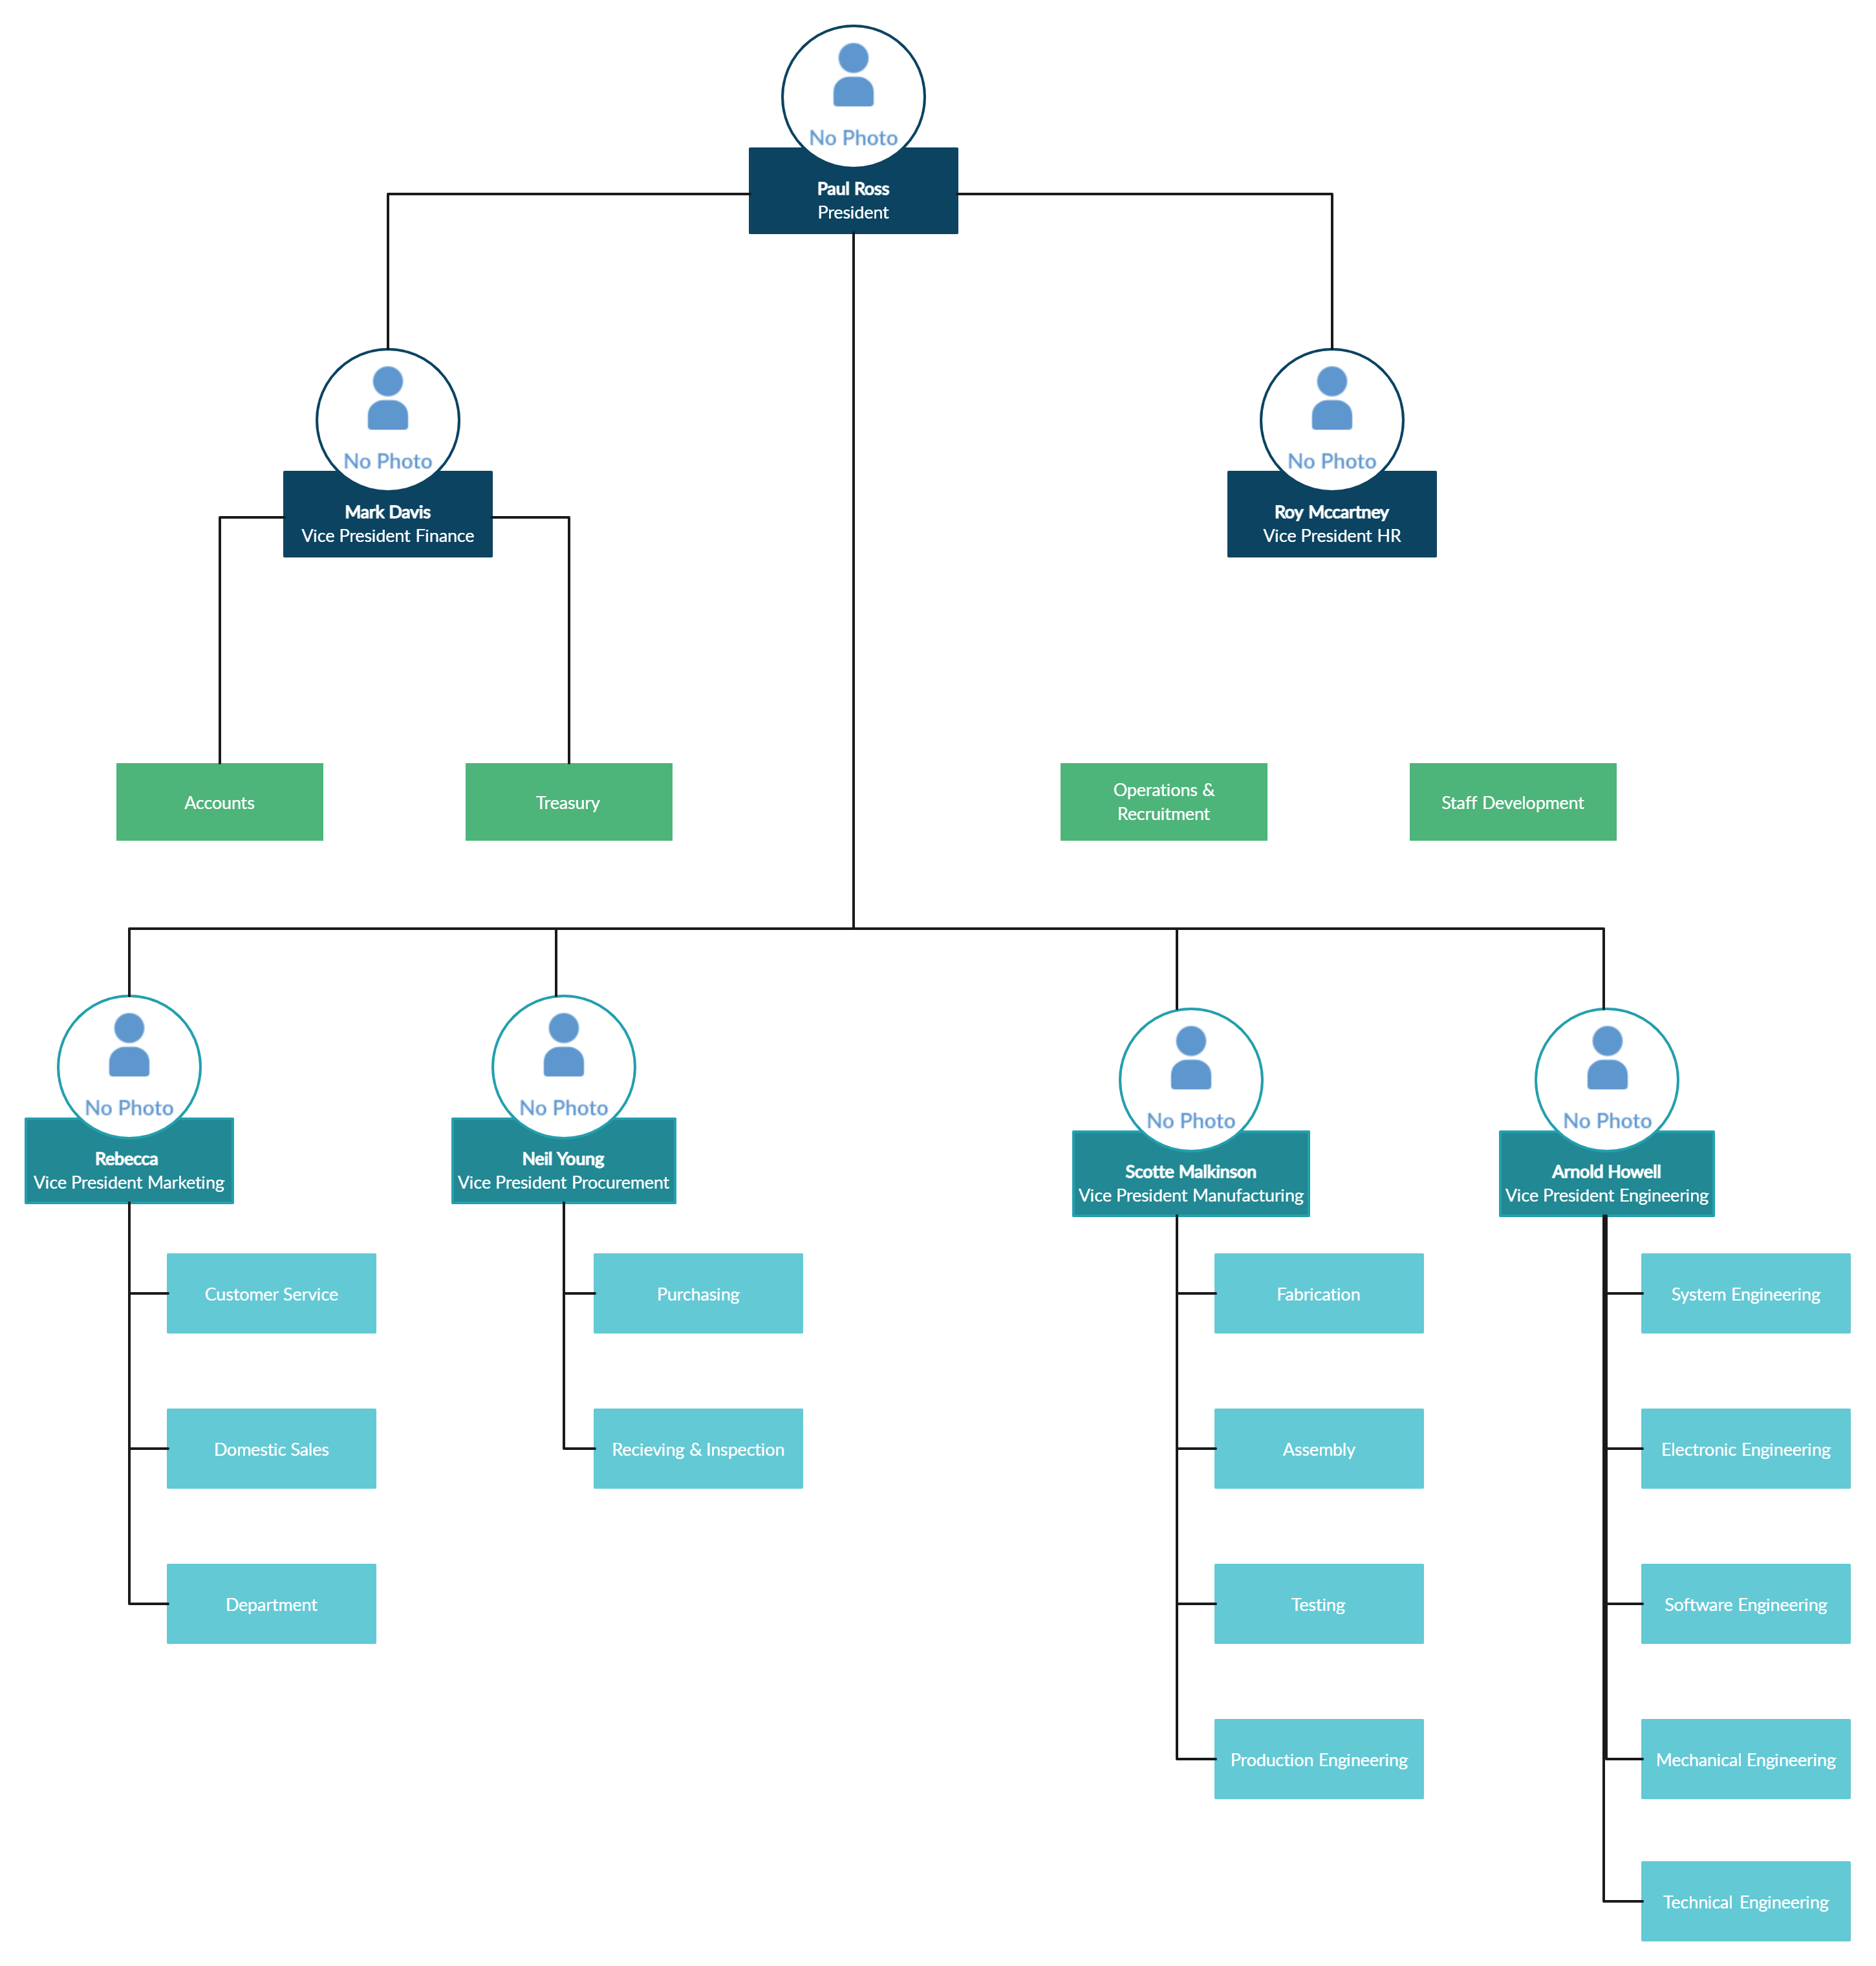
\includegraphics[width=12cm]{Figures/Organizational_Chart.png}
    \caption{Organizational Chart}
    %\label{fig:my_label} %Optional (If you want to reference the figure in later chapters)
\end{figure}











\section{Presentation of the project}


\subsection{Project Framework}



\subsection{Project objectives}





\subsection{Project Planning}

\begin{figure}[H] 
    \centering
    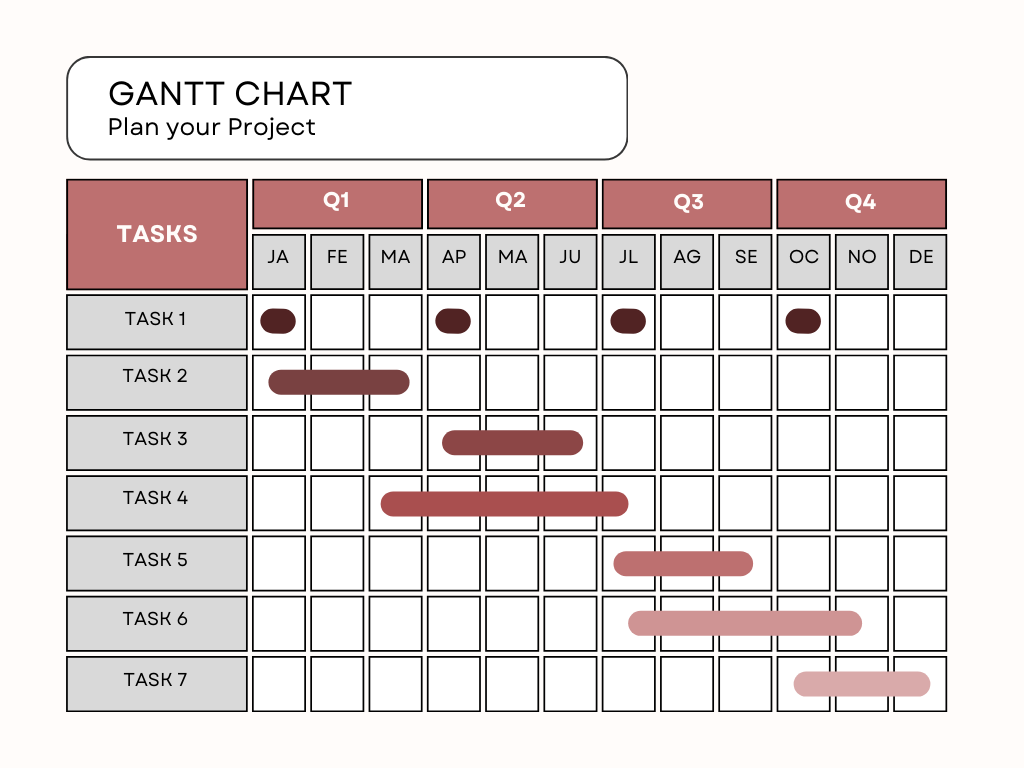
\includegraphics[width=12cm]{Figures/Gantt_Diagram.png}
    \caption{Gantt Diagram}
    %\label{fig:my_label} %Optional (If you want to reference the figure in later chapters)
\end{figure}

\newpage

\section*{Conclusion}

Lorem ipsum dolor sit amet, consectetur adipiscing elit. Praesent nec dapibus justo. Donec sagittis vulputate ante sed porttitor. Suspendisse sit amet nisl massa. Curabitur nec nisl condimentum, egestas ex vitae, dapibus enim. Etiam iaculis, erat faucibus pellentesque sagittis, nisi justo sollicitudin nibh, et condimentum augue massa non turpis. Proin commodo enim fermentum suscipit condimentum. Maecenas molestie, dui nec vestibulum rhoncus, arcu nisl faucibus neque, a ornare nisi massa ac eros. Aenean id velit sit amet lacus mattis varius. Donec fringilla massa sed nisi eleifend, a aliquet mi tempus. Nunc posuere euismod est, nec tristique augue lobortis non. Sed sodales sem ut metus tempus ullamcorper.
 for example. 

Remember to change the PDF Title and author name before the begin document command.
\\

Packages.tex is where you import packages and could modify their options.
\\

The frontmatter folder contains unnumbered chapters that come before the actual chapters, so the resumes and acknowledgments are there. The pages are numbered in Roman numbers.
\\

The chapters folder obviously contains the main chapters of the report, usually the first one is an intro, of both the project and the company, the last one is a conclusion chapter, I made it unnumbered here but you do you.
\\

The endmatter folder contains the appendices, acronyms, glossary, and Complementary figures, tables and codes. Consider checking this link \url{https://libguides.usc.edu/writingguide/appendices} for more info. Usually you add an appendix for each subject you'll talk about it, each with its own codes, tables, figures and text.
\\

The bibliography can be found at the end of main.tex file.
\\

And to organise your figures better, upload the logos to the logos folder, and content related figures should go in the figures folder, where you can add sub folders.
\\

Along the template, make sure to read my comments, they can be helpful to understand the purpose of a command or option. 
\\

When you finish writing your thesis, make sure to verify that you didn't leave any generic line or link. Revise it well.
\\

There are 10 warnings that show up in this template, some I couldn't manage to solve (or understand), and some I left since they are necessary for what I intend of this template.
\\

Obviously this template is only a suggestion, it is not perfect in any sense, you can improve it in the way that suits you, so search away, and get used to reading the documentation.
\\

Also consult with your supervisor, as each teacher has their own opinion on what constitutes the ideal report.
\\

Finally, I hope you have enjoyed your time at INPT as much as I did, and Good Luck :D
\\

-Mery


\subsection{Codes\_Needed}

This subsection includes codes for different elements you will need: figures, tables, lists...

Copy the codes you want and test them in the chapter files.

if you want symbols and other text styles, visit this link: 

\href{https://www.cmor-faculty.rice.edu/~heinken/latex/symbols.pdf}{Symbols}

Read the comments !!

% Content division

%\chapter{Comes first}, then \section{}, then \subsection{}, then \subsubsection{}.

\subsubsection{Text formatting}

\textbf{This text is bold}

\textit{This text is italic}

\underline{This text is underlined.}

\st{This text is struck out.}

\textsc{This text is capitalized.}

%Use \paragraph{To start a paragraph}


Some characters like "\%", "\$" and "\&" are significant in Latex code, so to include them in normal text, use the backslash character before them.
To print out backslash, use \symbol{92}


Documentation: \href{https://www.overleaf.com/learn/latex/Bold%2C_italics_and_underlining}{Italics and underlining}


\subsubsection{Figures} 

\begin{figure}[H] 
    \centering
    
\includegraphics[width=4cm]{Logos/Logo_INPT.png}
    \caption{Caption}
    \label{fig:my_label} %Optional (If you want to reference the figure in later chapters)
\end{figure}

%[width=7cm] you control the size of the image. other options include: 
%[height=7cm] or [scale=0.5] (means half the size of the original image)


Documentation: \href{https://www.overleaf.com/learn/latex/Inserting_Images}{Images}


\subsubsection{Tables} 

Simple table without borders:
\\

\begin{tabular}{ll}
  First & Second \\
  Third & Fourth
\end{tabular}
\\

More complex table with borders:
\\

\begin{tabular}{|l|c|r|} \hline
  Left aligned column & Centered column & Right aligned column \\ \hline
  Text & Text & Text \\ \hline
\end{tabular}
\\

Example of a short table

%{5cm} is the cell length, you can change it to suit your own table

\begin{table}[H]
    \centering
    \begin{tabular}{|m{5cm}|m{10cm}|}
        \hline
          Column1 & Column2 \\
        \hline
          Element11 & Element21 \\
        \hline
          Element12 & Element22 \\
        \hline
          Element13 & Element23 \\
        \hline
    \end{tabular}
    \caption{Table Example}
\end{table}


Example of a long table (that spans 2 pages or more), Latex will automatically split the table when it reaches the end of the page:

\begin{longtable}[c]{| m{4.4cm} | m{11cm} |}
\caption{Long table}\\
 \hline

 Cell & Description  \\ 
 \hline
 \endfirsthead

 \hline
 
 Cell & Description  \\ 
 \hline
 \endhead

        \hline
          Element11 & Element21 \\
        \hline
          Element12 & Element22 \\
        \hline
          Element13 & Element23 \\
        \hline
          Element14 & Element24 \\
        \hline
          Element15 & Element25 \\
        \hline
          Element16 & Element26 \\
        \hline
          Element17 & Element27 \\
        \hline
          Element18 & Element28 \\
        \hline
          Element19 & Element29 \\
        \hline
          Element110 & Element210 \\
        \hline
          Element111 & Element211 \\
        \hline
          Element112 & Element212 \\
        \hline
          Element113 & Element213 \\
        \hline
          Element114 & Element214 \\
        \hline

 \end{longtable}


Documentation: \href{https://www.overleaf.com/learn/latex/Tables}{Tables}


\subsubsection{Lists}

To start an unnumbered list, use:

\begin{itemize}
    \item 
    \item 
    \item 
\end{itemize}

To start a numbered list, use:

\begin{enumerate}
    \item 
    \item 
    \item 
\end{enumerate}



Documentation: \href{https://www.overleaf.com/learn/latex/Lists}{Lists}


\subsubsection{Code scripts or terminal}

Say you have a script or terminal command you want to include, you use the following code:

    \lstset{style=mystyle} %this style is already defined in Packages.tex
    
    \begin{lstlisting}[language=bash, caption= Code caption]
    
    root@eve-ng:~# mkdir -p /opt/unetlab/addons/qemu/timos-20.10.R12

    \end{lstlisting}


Documentation: \href{https://www.overleaf.com/learn/latex/Code_listing}{Code Listing}

\subsubsection{Math}

Some math formulas for you, test them in your chapters:

These are inline formulas: $x$, $a_i^2 + b_i^2 \le a_{i+1}^2$. Afterwards...

These are centered formulas: $$x,$$ $$a_i^2 + b_i^2 \le a_{i+1}^2.$$ Afterwards...

Some complex formula: $$P(|S - E[S]| \ge t) \le 2 \exp \left( -\frac{2 t^2 n^2}{\sum_{i = 1}^n (b_i - a_i)^2} \right).$$

Also you can use the first link for math symbols and other useful stuff:

Documentation: \href{https://www.cmor-faculty.rice.edu/~heinken/latex/symbols.pdf}{Symbols file again}



\newpage


\section{Presentation of host organization}



\subsection{Company Overview}

\begin{figure}[H] 
    \centering
    \includegraphics[width=7cm]{Logos/Company_Logo_Expl.png}
    \caption{Company logo}
    %\label{fig:my_label} %Optional (If you want to reference the figure in later chapters)
\end{figure}



\subsection{Organizational Chart}


\begin{figure}[H] 
    \centering
    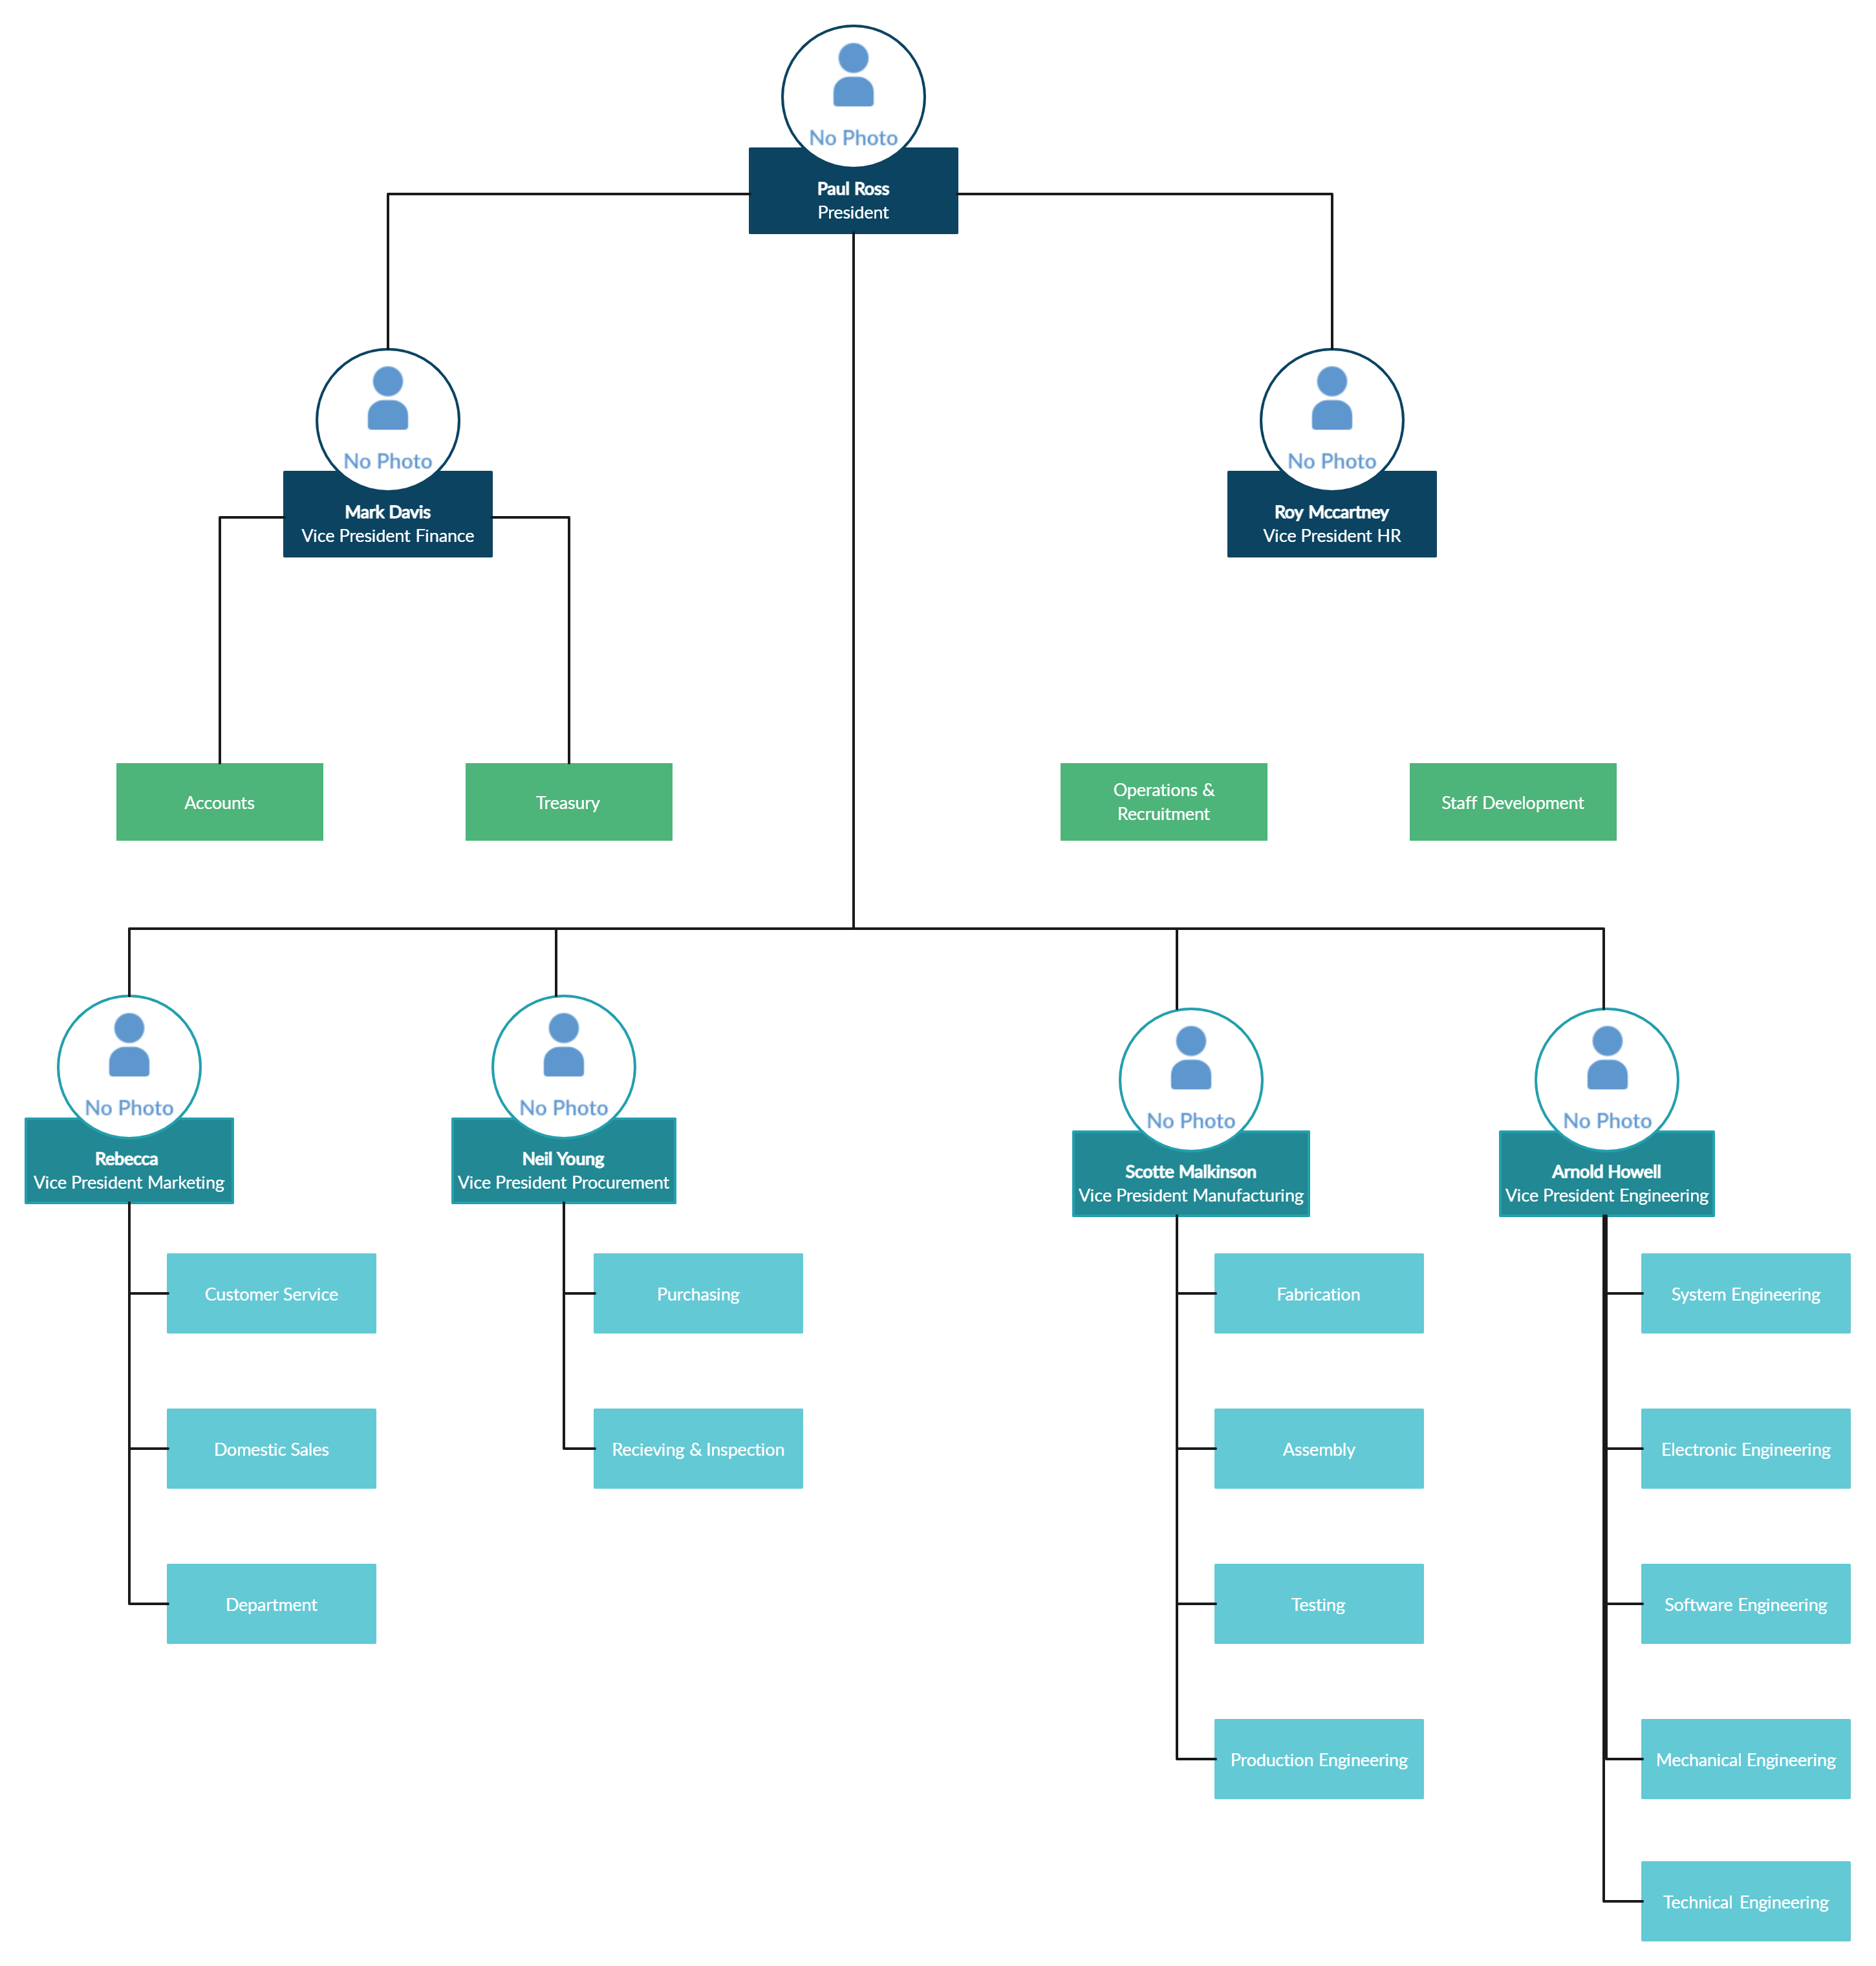
\includegraphics[width=12cm]{Figures/Organizational_Chart.png}
    \caption{Organizational Chart}
    %\label{fig:my_label} %Optional (If you want to reference the figure in later chapters)
\end{figure}











\section{Presentation of the project}


\subsection{Project Framework}



\subsection{Project objectives}





\subsection{Project Planning}

\begin{figure}[H] 
    \centering
    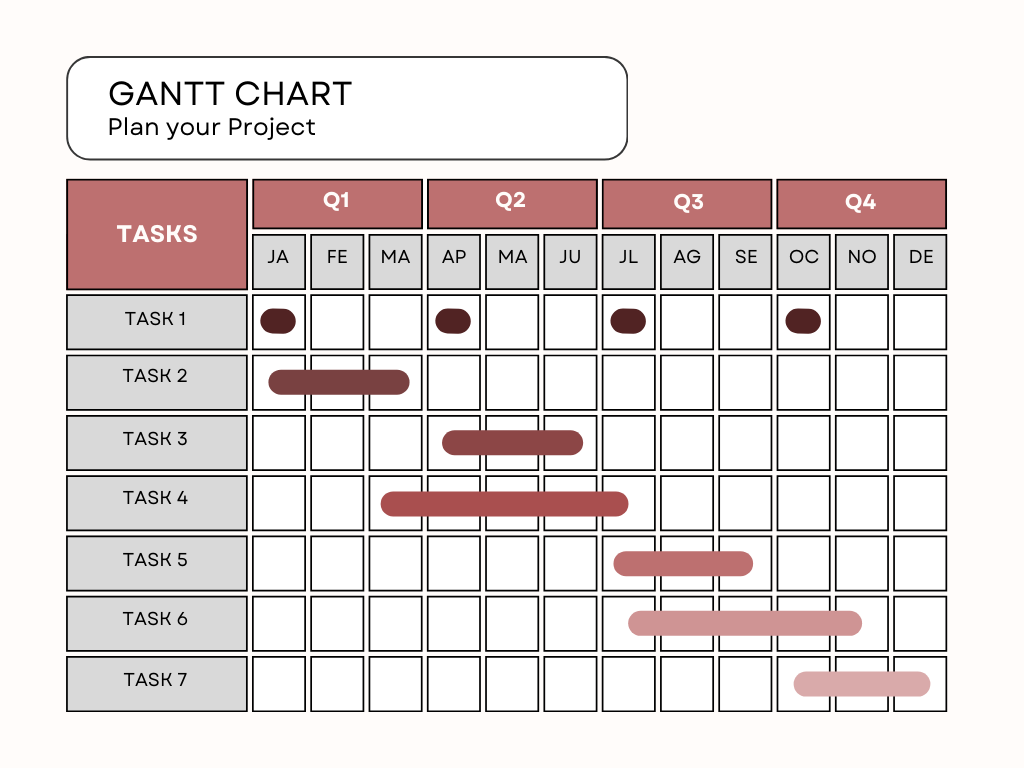
\includegraphics[width=12cm]{Figures/Gantt_Diagram.png}
    \caption{Gantt Diagram}
    %\label{fig:my_label} %Optional (If you want to reference the figure in later chapters)
\end{figure}

\newpage

\section*{Conclusion}

Lorem ipsum dolor sit amet, consectetur adipiscing elit. Praesent nec dapibus justo. Donec sagittis vulputate ante sed porttitor. Suspendisse sit amet nisl massa. Curabitur nec nisl condimentum, egestas ex vitae, dapibus enim. Etiam iaculis, erat faucibus pellentesque sagittis, nisi justo sollicitudin nibh, et condimentum augue massa non turpis. Proin commodo enim fermentum suscipit condimentum. Maecenas molestie, dui nec vestibulum rhoncus, arcu nisl faucibus neque, a ornare nisi massa ac eros. Aenean id velit sit amet lacus mattis varius. Donec fringilla massa sed nisi eleifend, a aliquet mi tempus. Nunc posuere euismod est, nec tristique augue lobortis non. Sed sodales sem ut metus tempus ullamcorper.
 for example. 

Remember to change the PDF Title and author name before the begin document command.
\\

Packages.tex is where you import packages and could modify their options.
\\

The frontmatter folder contains unnumbered chapters that come before the actual chapters, so the resumes and acknowledgments are there. The pages are numbered in Roman numbers.
\\

The chapters folder obviously contains the main chapters of the report, usually the first one is an intro, of both the project and the company, the last one is a conclusion chapter, I made it unnumbered here but you do you.
\\

The endmatter folder contains the appendices, acronyms, glossary, and Complementary figures, tables and codes. Consider checking this link \url{https://libguides.usc.edu/writingguide/appendices} for more info. Usually you add an appendix for each subject you'll talk about it, each with its own codes, tables, figures and text.
\\

The bibliography can be found at the end of main.tex file.
\\

And to organise your figures better, upload the logos to the logos folder, and content related figures should go in the figures folder, where you can add sub folders.
\\

Along the template, make sure to read my comments, they can be helpful to understand the purpose of a command or option. 
\\

When you finish writing your thesis, make sure to verify that you didn't leave any generic line or link. Revise it well.
\\

There are 10 warnings that show up in this template, some I couldn't manage to solve (or understand), and some I left since they are necessary for what I intend of this template.
\\

Obviously this template is only a suggestion, it is not perfect in any sense, you can improve it in the way that suits you, so search away, and get used to reading the documentation.
\\

Also consult with your supervisor, as each teacher has their own opinion on what constitutes the ideal report.
\\

Finally, I hope you have enjoyed your time at INPT as much as I did, and Good Luck :D
\\

-Mery


\subsection{Codes\_Needed}

This subsection includes codes for different elements you will need: figures, tables, lists...

Copy the codes you want and test them in the chapter files.

if you want symbols and other text styles, visit this link: 

\href{https://www.cmor-faculty.rice.edu/~heinken/latex/symbols.pdf}{Symbols}

Read the comments !!

% Content division

%\chapter{Comes first}, then \section{}, then \subsection{}, then \subsubsection{}.

\subsubsection{Text formatting}

\textbf{This text is bold}

\textit{This text is italic}

\underline{This text is underlined.}

\st{This text is struck out.}

\textsc{This text is capitalized.}

%Use \paragraph{To start a paragraph}


Some characters like "\%", "\$" and "\&" are significant in Latex code, so to include them in normal text, use the backslash character before them.
To print out backslash, use \symbol{92}


Documentation: \href{https://www.overleaf.com/learn/latex/Bold%2C_italics_and_underlining}{Italics and underlining}


\subsubsection{Figures} 

\begin{figure}[H] 
    \centering
    
\includegraphics[width=4cm]{Logos/Logo_INPT.png}
    \caption{Caption}
    \label{fig:my_label} %Optional (If you want to reference the figure in later chapters)
\end{figure}

%[width=7cm] you control the size of the image. other options include: 
%[height=7cm] or [scale=0.5] (means half the size of the original image)


Documentation: \href{https://www.overleaf.com/learn/latex/Inserting_Images}{Images}


\subsubsection{Tables} 

Simple table without borders:
\\

\begin{tabular}{ll}
  First & Second \\
  Third & Fourth
\end{tabular}
\\

More complex table with borders:
\\

\begin{tabular}{|l|c|r|} \hline
  Left aligned column & Centered column & Right aligned column \\ \hline
  Text & Text & Text \\ \hline
\end{tabular}
\\

Example of a short table

%{5cm} is the cell length, you can change it to suit your own table

\begin{table}[H]
    \centering
    \begin{tabular}{|m{5cm}|m{10cm}|}
        \hline
          Column1 & Column2 \\
        \hline
          Element11 & Element21 \\
        \hline
          Element12 & Element22 \\
        \hline
          Element13 & Element23 \\
        \hline
    \end{tabular}
    \caption{Table Example}
\end{table}


Example of a long table (that spans 2 pages or more), Latex will automatically split the table when it reaches the end of the page:

\begin{longtable}[c]{| m{4.4cm} | m{11cm} |}
\caption{Long table}\\
 \hline

 Cell & Description  \\ 
 \hline
 \endfirsthead

 \hline
 
 Cell & Description  \\ 
 \hline
 \endhead

        \hline
          Element11 & Element21 \\
        \hline
          Element12 & Element22 \\
        \hline
          Element13 & Element23 \\
        \hline
          Element14 & Element24 \\
        \hline
          Element15 & Element25 \\
        \hline
          Element16 & Element26 \\
        \hline
          Element17 & Element27 \\
        \hline
          Element18 & Element28 \\
        \hline
          Element19 & Element29 \\
        \hline
          Element110 & Element210 \\
        \hline
          Element111 & Element211 \\
        \hline
          Element112 & Element212 \\
        \hline
          Element113 & Element213 \\
        \hline
          Element114 & Element214 \\
        \hline

 \end{longtable}


Documentation: \href{https://www.overleaf.com/learn/latex/Tables}{Tables}


\subsubsection{Lists}

To start an unnumbered list, use:

\begin{itemize}
    \item 
    \item 
    \item 
\end{itemize}

To start a numbered list, use:

\begin{enumerate}
    \item 
    \item 
    \item 
\end{enumerate}



Documentation: \href{https://www.overleaf.com/learn/latex/Lists}{Lists}


\subsubsection{Code scripts or terminal}

Say you have a script or terminal command you want to include, you use the following code:

    \lstset{style=mystyle} %this style is already defined in Packages.tex
    
    \begin{lstlisting}[language=bash, caption= Code caption]
    
    root@eve-ng:~# mkdir -p /opt/unetlab/addons/qemu/timos-20.10.R12

    \end{lstlisting}


Documentation: \href{https://www.overleaf.com/learn/latex/Code_listing}{Code Listing}

\subsubsection{Math}

Some math formulas for you, test them in your chapters:

These are inline formulas: $x$, $a_i^2 + b_i^2 \le a_{i+1}^2$. Afterwards...

These are centered formulas: $$x,$$ $$a_i^2 + b_i^2 \le a_{i+1}^2.$$ Afterwards...

Some complex formula: $$P(|S - E[S]| \ge t) \le 2 \exp \left( -\frac{2 t^2 n^2}{\sum_{i = 1}^n (b_i - a_i)^2} \right).$$

Also you can use the first link for math symbols and other useful stuff:

Documentation: \href{https://www.cmor-faculty.rice.edu/~heinken/latex/symbols.pdf}{Symbols file again}



\newpage


\section{Presentation of host organization}



\subsection{Company Overview}

\begin{figure}[H] 
    \centering
    \includegraphics[width=7cm]{Logos/Company_Logo_Expl.png}
    \caption{Company logo}
    %\label{fig:my_label} %Optional (If you want to reference the figure in later chapters)
\end{figure}



\subsection{Organizational Chart}


\begin{figure}[H] 
    \centering
    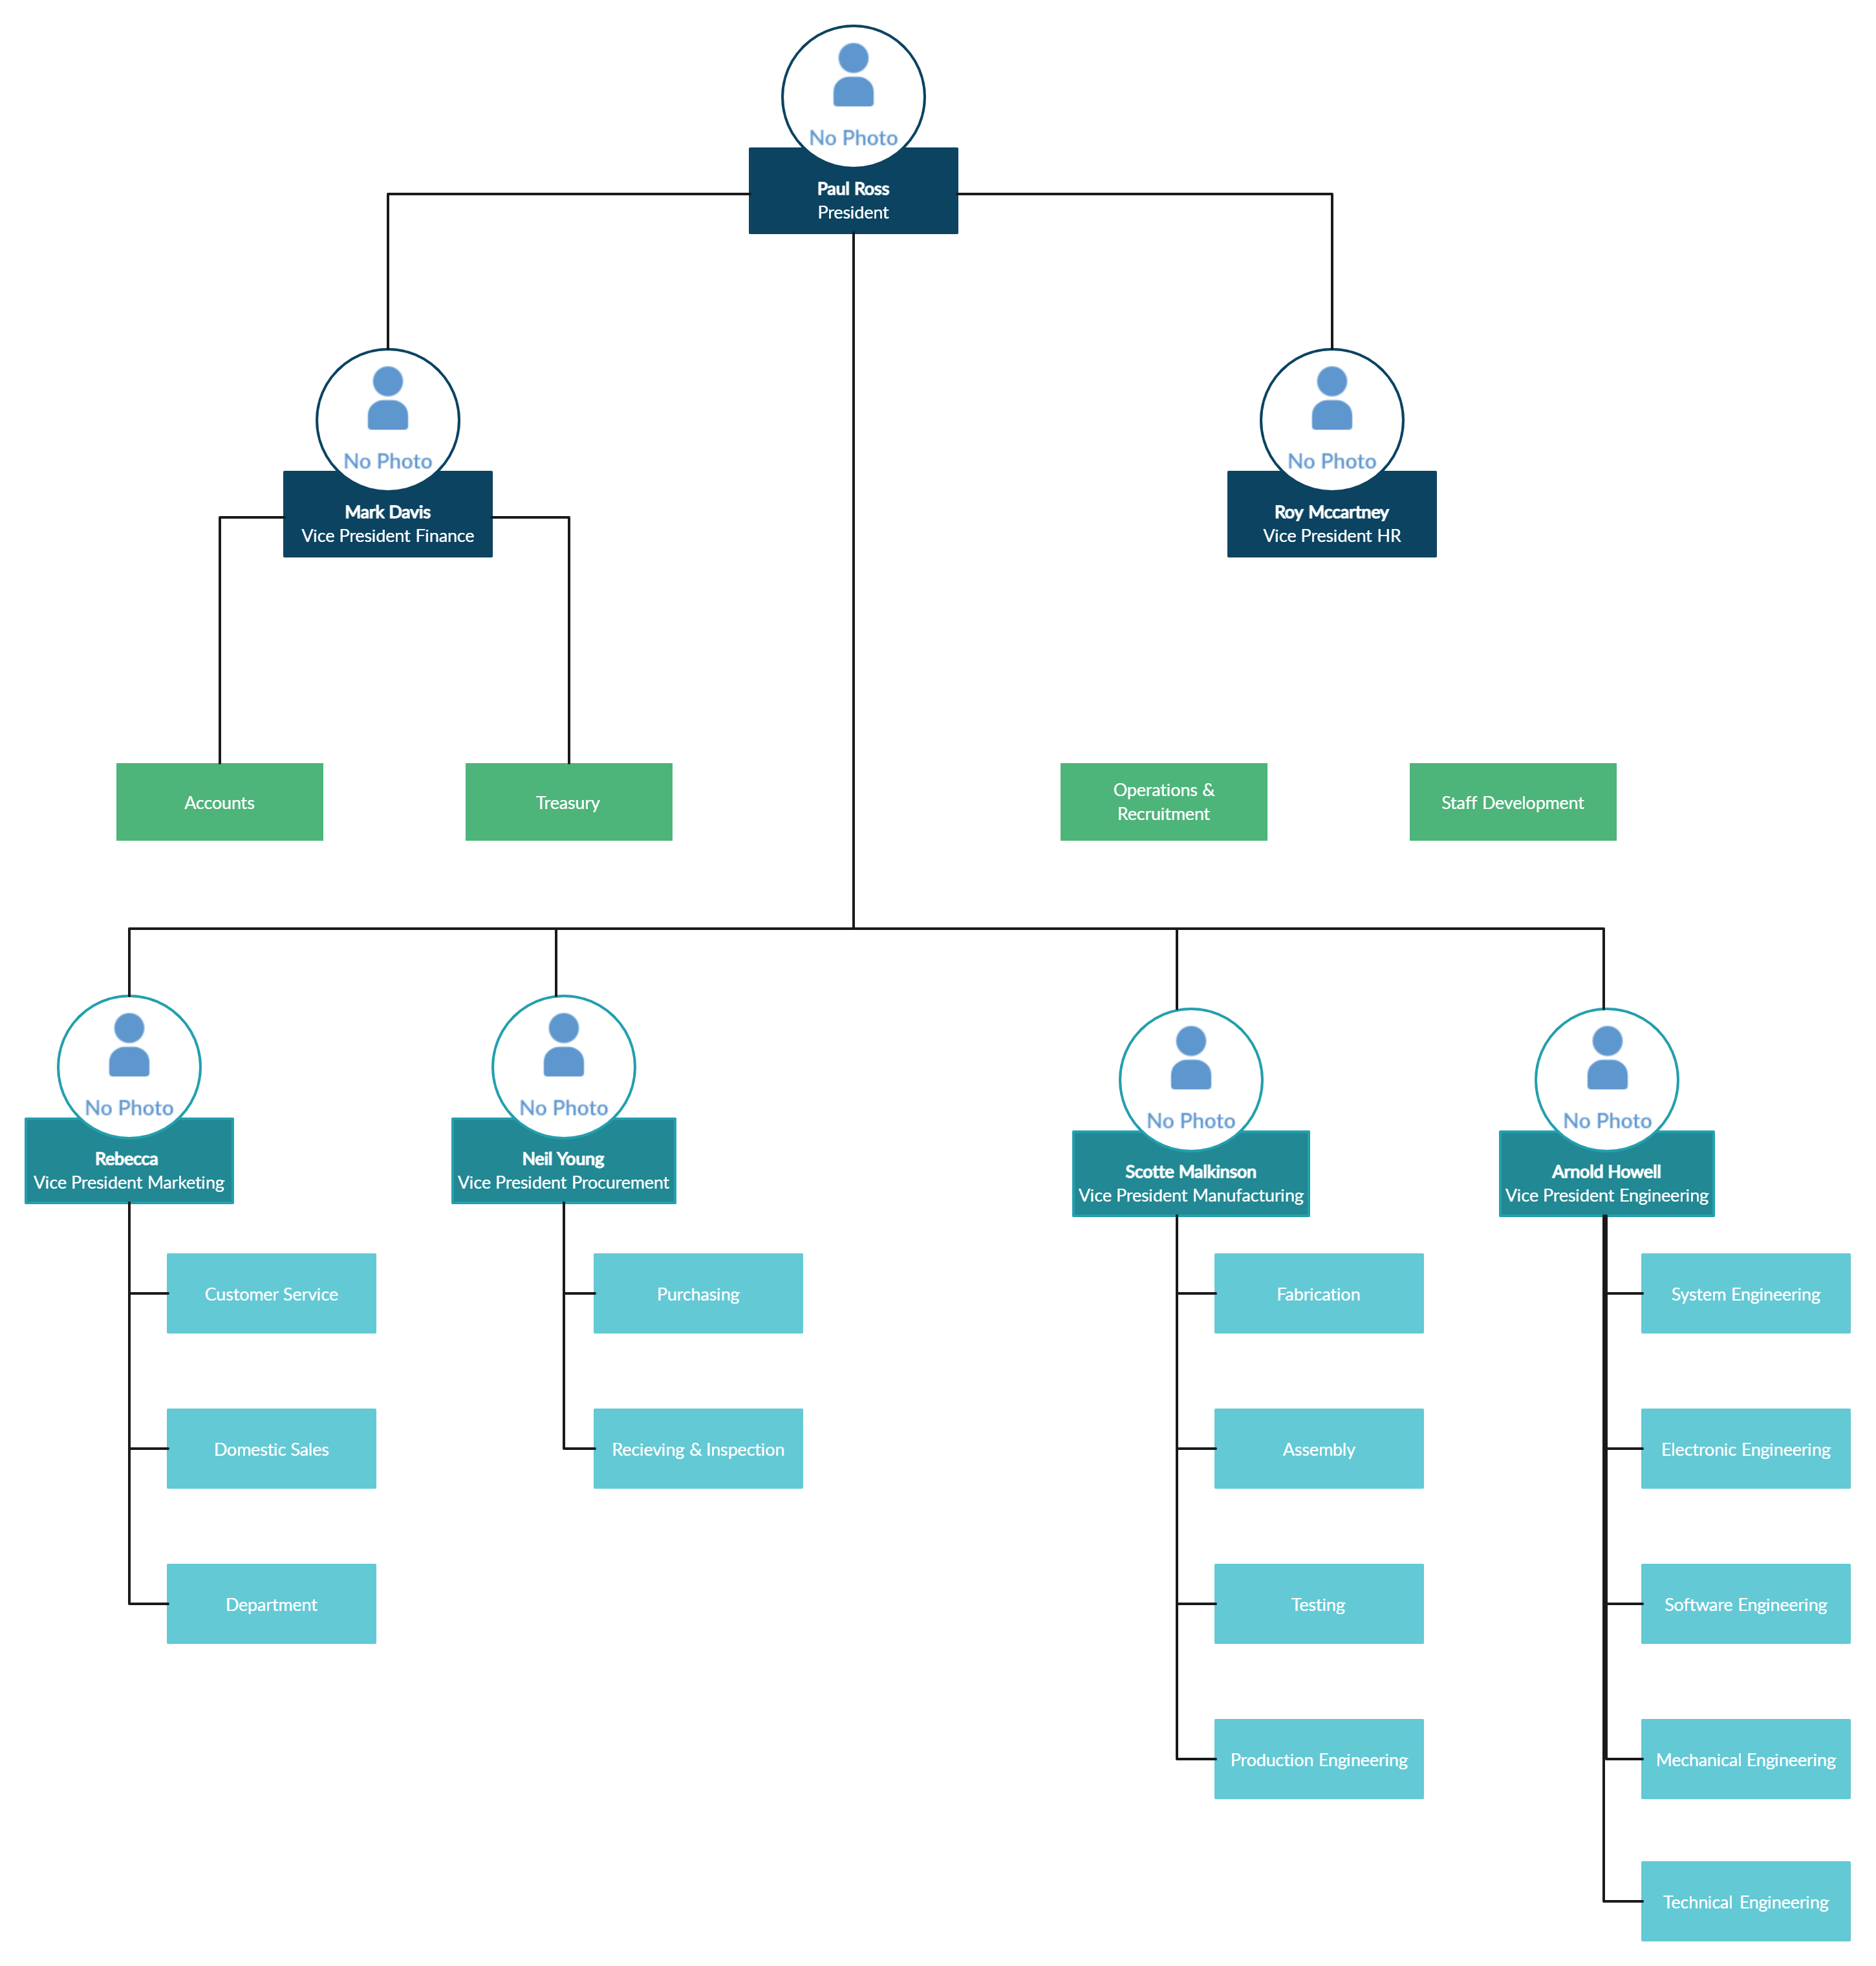
\includegraphics[width=12cm]{Figures/Organizational_Chart.png}
    \caption{Organizational Chart}
    %\label{fig:my_label} %Optional (If you want to reference the figure in later chapters)
\end{figure}











\section{Presentation of the project}


\subsection{Project Framework}



\subsection{Project objectives}





\subsection{Project Planning}

\begin{figure}[H] 
    \centering
    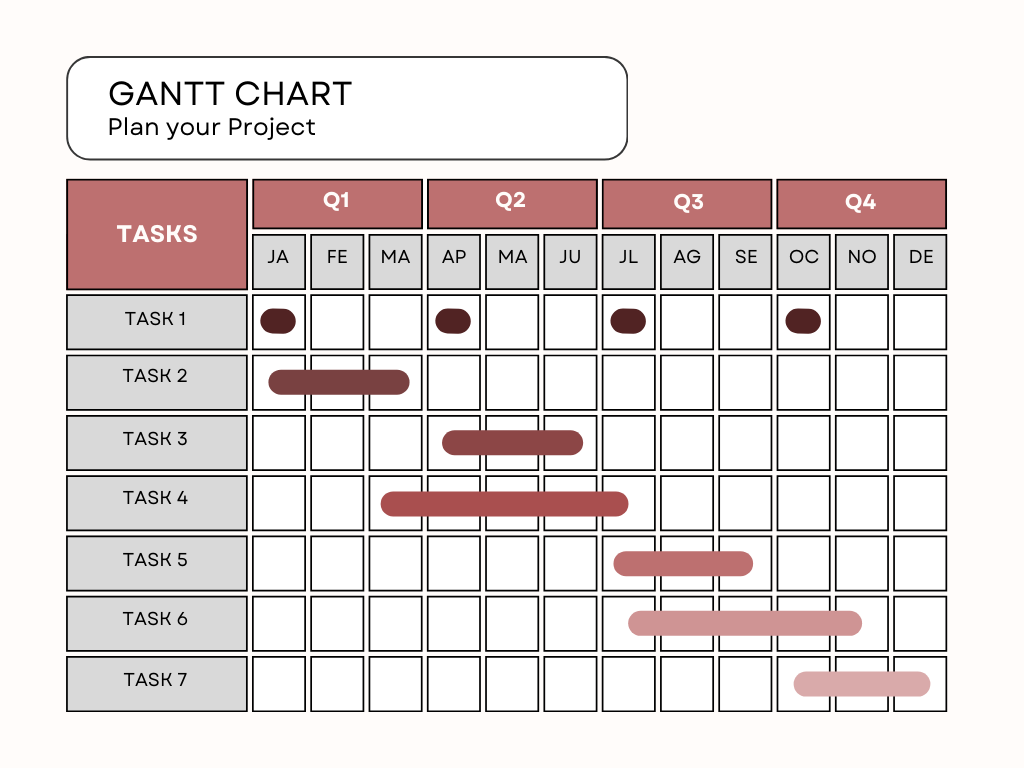
\includegraphics[width=12cm]{Figures/Gantt_Diagram.png}
    \caption{Gantt Diagram}
    %\label{fig:my_label} %Optional (If you want to reference the figure in later chapters)
\end{figure}

\newpage

\section*{Conclusion}

Lorem ipsum dolor sit amet, consectetur adipiscing elit. Praesent nec dapibus justo. Donec sagittis vulputate ante sed porttitor. Suspendisse sit amet nisl massa. Curabitur nec nisl condimentum, egestas ex vitae, dapibus enim. Etiam iaculis, erat faucibus pellentesque sagittis, nisi justo sollicitudin nibh, et condimentum augue massa non turpis. Proin commodo enim fermentum suscipit condimentum. Maecenas molestie, dui nec vestibulum rhoncus, arcu nisl faucibus neque, a ornare nisi massa ac eros. Aenean id velit sit amet lacus mattis varius. Donec fringilla massa sed nisi eleifend, a aliquet mi tempus. Nunc posuere euismod est, nec tristique augue lobortis non. Sed sodales sem ut metus tempus ullamcorper.
 for example. 

Remember to change the PDF Title and author name before the begin document command.
\\

Packages.tex is where you import packages and could modify their options.
\\

The frontmatter folder contains unnumbered chapters that come before the actual chapters, so the resumes and acknowledgments are there. The pages are numbered in Roman numbers.
\\

The chapters folder obviously contains the main chapters of the report, usually the first one is an intro, of both the project and the company, the last one is a conclusion chapter, I made it unnumbered here but you do you.
\\

The endmatter folder contains the appendices, acronyms, glossary, and Complementary figures, tables and codes. Consider checking this link \url{https://libguides.usc.edu/writingguide/appendices} for more info. Usually you add an appendix for each subject you'll talk about it, each with its own codes, tables, figures and text.
\\

The bibliography can be found at the end of main.tex file.
\\

And to organise your figures better, upload the logos to the logos folder, and content related figures should go in the figures folder, where you can add sub folders.
\\

Along the template, make sure to read my comments, they can be helpful to understand the purpose of a command or option. 
\\

When you finish writing your thesis, make sure to verify that you didn't leave any generic line or link. Revise it well.
\\

There are 10 warnings that show up in this template, some I couldn't manage to solve (or understand), and some I left since they are necessary for what I intend of this template.
\\

Obviously this template is only a suggestion, it is not perfect in any sense, you can improve it in the way that suits you, so search away, and get used to reading the documentation.
\\

Also consult with your supervisor, as each teacher has their own opinion on what constitutes the ideal report.
\\

Finally, I hope you have enjoyed your time at INPT as much as I did, and Good Luck :D
\\

-Mery


\subsection{Codes\_Needed}

This subsection includes codes for different elements you will need: figures, tables, lists...

Copy the codes you want and test them in the chapter files.

if you want symbols and other text styles, visit this link: 

\href{https://www.cmor-faculty.rice.edu/~heinken/latex/symbols.pdf}{Symbols}

Read the comments !!

% Content division

%\chapter{Comes first}, then \section{}, then \subsection{}, then \subsubsection{}.

\subsubsection{Text formatting}

\textbf{This text is bold}

\textit{This text is italic}

\underline{This text is underlined.}

\st{This text is struck out.}

\textsc{This text is capitalized.}

%Use \paragraph{To start a paragraph}


Some characters like "\%", "\$" and "\&" are significant in Latex code, so to include them in normal text, use the backslash character before them.
To print out backslash, use \symbol{92}


Documentation: \href{https://www.overleaf.com/learn/latex/Bold%2C_italics_and_underlining}{Italics and underlining}


\subsubsection{Figures} 

\begin{figure}[H] 
    \centering
    
\includegraphics[width=4cm]{Logos/Logo_INPT.png}
    \caption{Caption}
    \label{fig:my_label} %Optional (If you want to reference the figure in later chapters)
\end{figure}

%[width=7cm] you control the size of the image. other options include: 
%[height=7cm] or [scale=0.5] (means half the size of the original image)


Documentation: \href{https://www.overleaf.com/learn/latex/Inserting_Images}{Images}


\subsubsection{Tables} 

Simple table without borders:
\\

\begin{tabular}{ll}
  First & Second \\
  Third & Fourth
\end{tabular}
\\

More complex table with borders:
\\

\begin{tabular}{|l|c|r|} \hline
  Left aligned column & Centered column & Right aligned column \\ \hline
  Text & Text & Text \\ \hline
\end{tabular}
\\

Example of a short table

%{5cm} is the cell length, you can change it to suit your own table

\begin{table}[H]
    \centering
    \begin{tabular}{|m{5cm}|m{10cm}|}
        \hline
          Column1 & Column2 \\
        \hline
          Element11 & Element21 \\
        \hline
          Element12 & Element22 \\
        \hline
          Element13 & Element23 \\
        \hline
    \end{tabular}
    \caption{Table Example}
\end{table}


Example of a long table (that spans 2 pages or more), Latex will automatically split the table when it reaches the end of the page:

\begin{longtable}[c]{| m{4.4cm} | m{11cm} |}
\caption{Long table}\\
 \hline

 Cell & Description  \\ 
 \hline
 \endfirsthead

 \hline
 
 Cell & Description  \\ 
 \hline
 \endhead

        \hline
          Element11 & Element21 \\
        \hline
          Element12 & Element22 \\
        \hline
          Element13 & Element23 \\
        \hline
          Element14 & Element24 \\
        \hline
          Element15 & Element25 \\
        \hline
          Element16 & Element26 \\
        \hline
          Element17 & Element27 \\
        \hline
          Element18 & Element28 \\
        \hline
          Element19 & Element29 \\
        \hline
          Element110 & Element210 \\
        \hline
          Element111 & Element211 \\
        \hline
          Element112 & Element212 \\
        \hline
          Element113 & Element213 \\
        \hline
          Element114 & Element214 \\
        \hline

 \end{longtable}


Documentation: \href{https://www.overleaf.com/learn/latex/Tables}{Tables}


\subsubsection{Lists}

To start an unnumbered list, use:

\begin{itemize}
    \item 
    \item 
    \item 
\end{itemize}

To start a numbered list, use:

\begin{enumerate}
    \item 
    \item 
    \item 
\end{enumerate}



Documentation: \href{https://www.overleaf.com/learn/latex/Lists}{Lists}


\subsubsection{Code scripts or terminal}

Say you have a script or terminal command you want to include, you use the following code:

    \lstset{style=mystyle} %this style is already defined in Packages.tex
    
    \begin{lstlisting}[language=bash, caption= Code caption]
    
    root@eve-ng:~# mkdir -p /opt/unetlab/addons/qemu/timos-20.10.R12

    \end{lstlisting}


Documentation: \href{https://www.overleaf.com/learn/latex/Code_listing}{Code Listing}

\subsubsection{Math}

Some math formulas for you, test them in your chapters:

These are inline formulas: $x$, $a_i^2 + b_i^2 \le a_{i+1}^2$. Afterwards...

These are centered formulas: $$x,$$ $$a_i^2 + b_i^2 \le a_{i+1}^2.$$ Afterwards...

Some complex formula: $$P(|S - E[S]| \ge t) \le 2 \exp \left( -\frac{2 t^2 n^2}{\sum_{i = 1}^n (b_i - a_i)^2} \right).$$

Also you can use the first link for math symbols and other useful stuff:

Documentation: \href{https://www.cmor-faculty.rice.edu/~heinken/latex/symbols.pdf}{Symbols file again}



\newpage


\section{Presentation of host organization}



\subsection{Company Overview}

\begin{figure}[H] 
    \centering
    \includegraphics[width=7cm]{Logos/Company_Logo_Expl.png}
    \caption{Company logo}
    %\label{fig:my_label} %Optional (If you want to reference the figure in later chapters)
\end{figure}



\subsection{Organizational Chart}


\begin{figure}[H] 
    \centering
    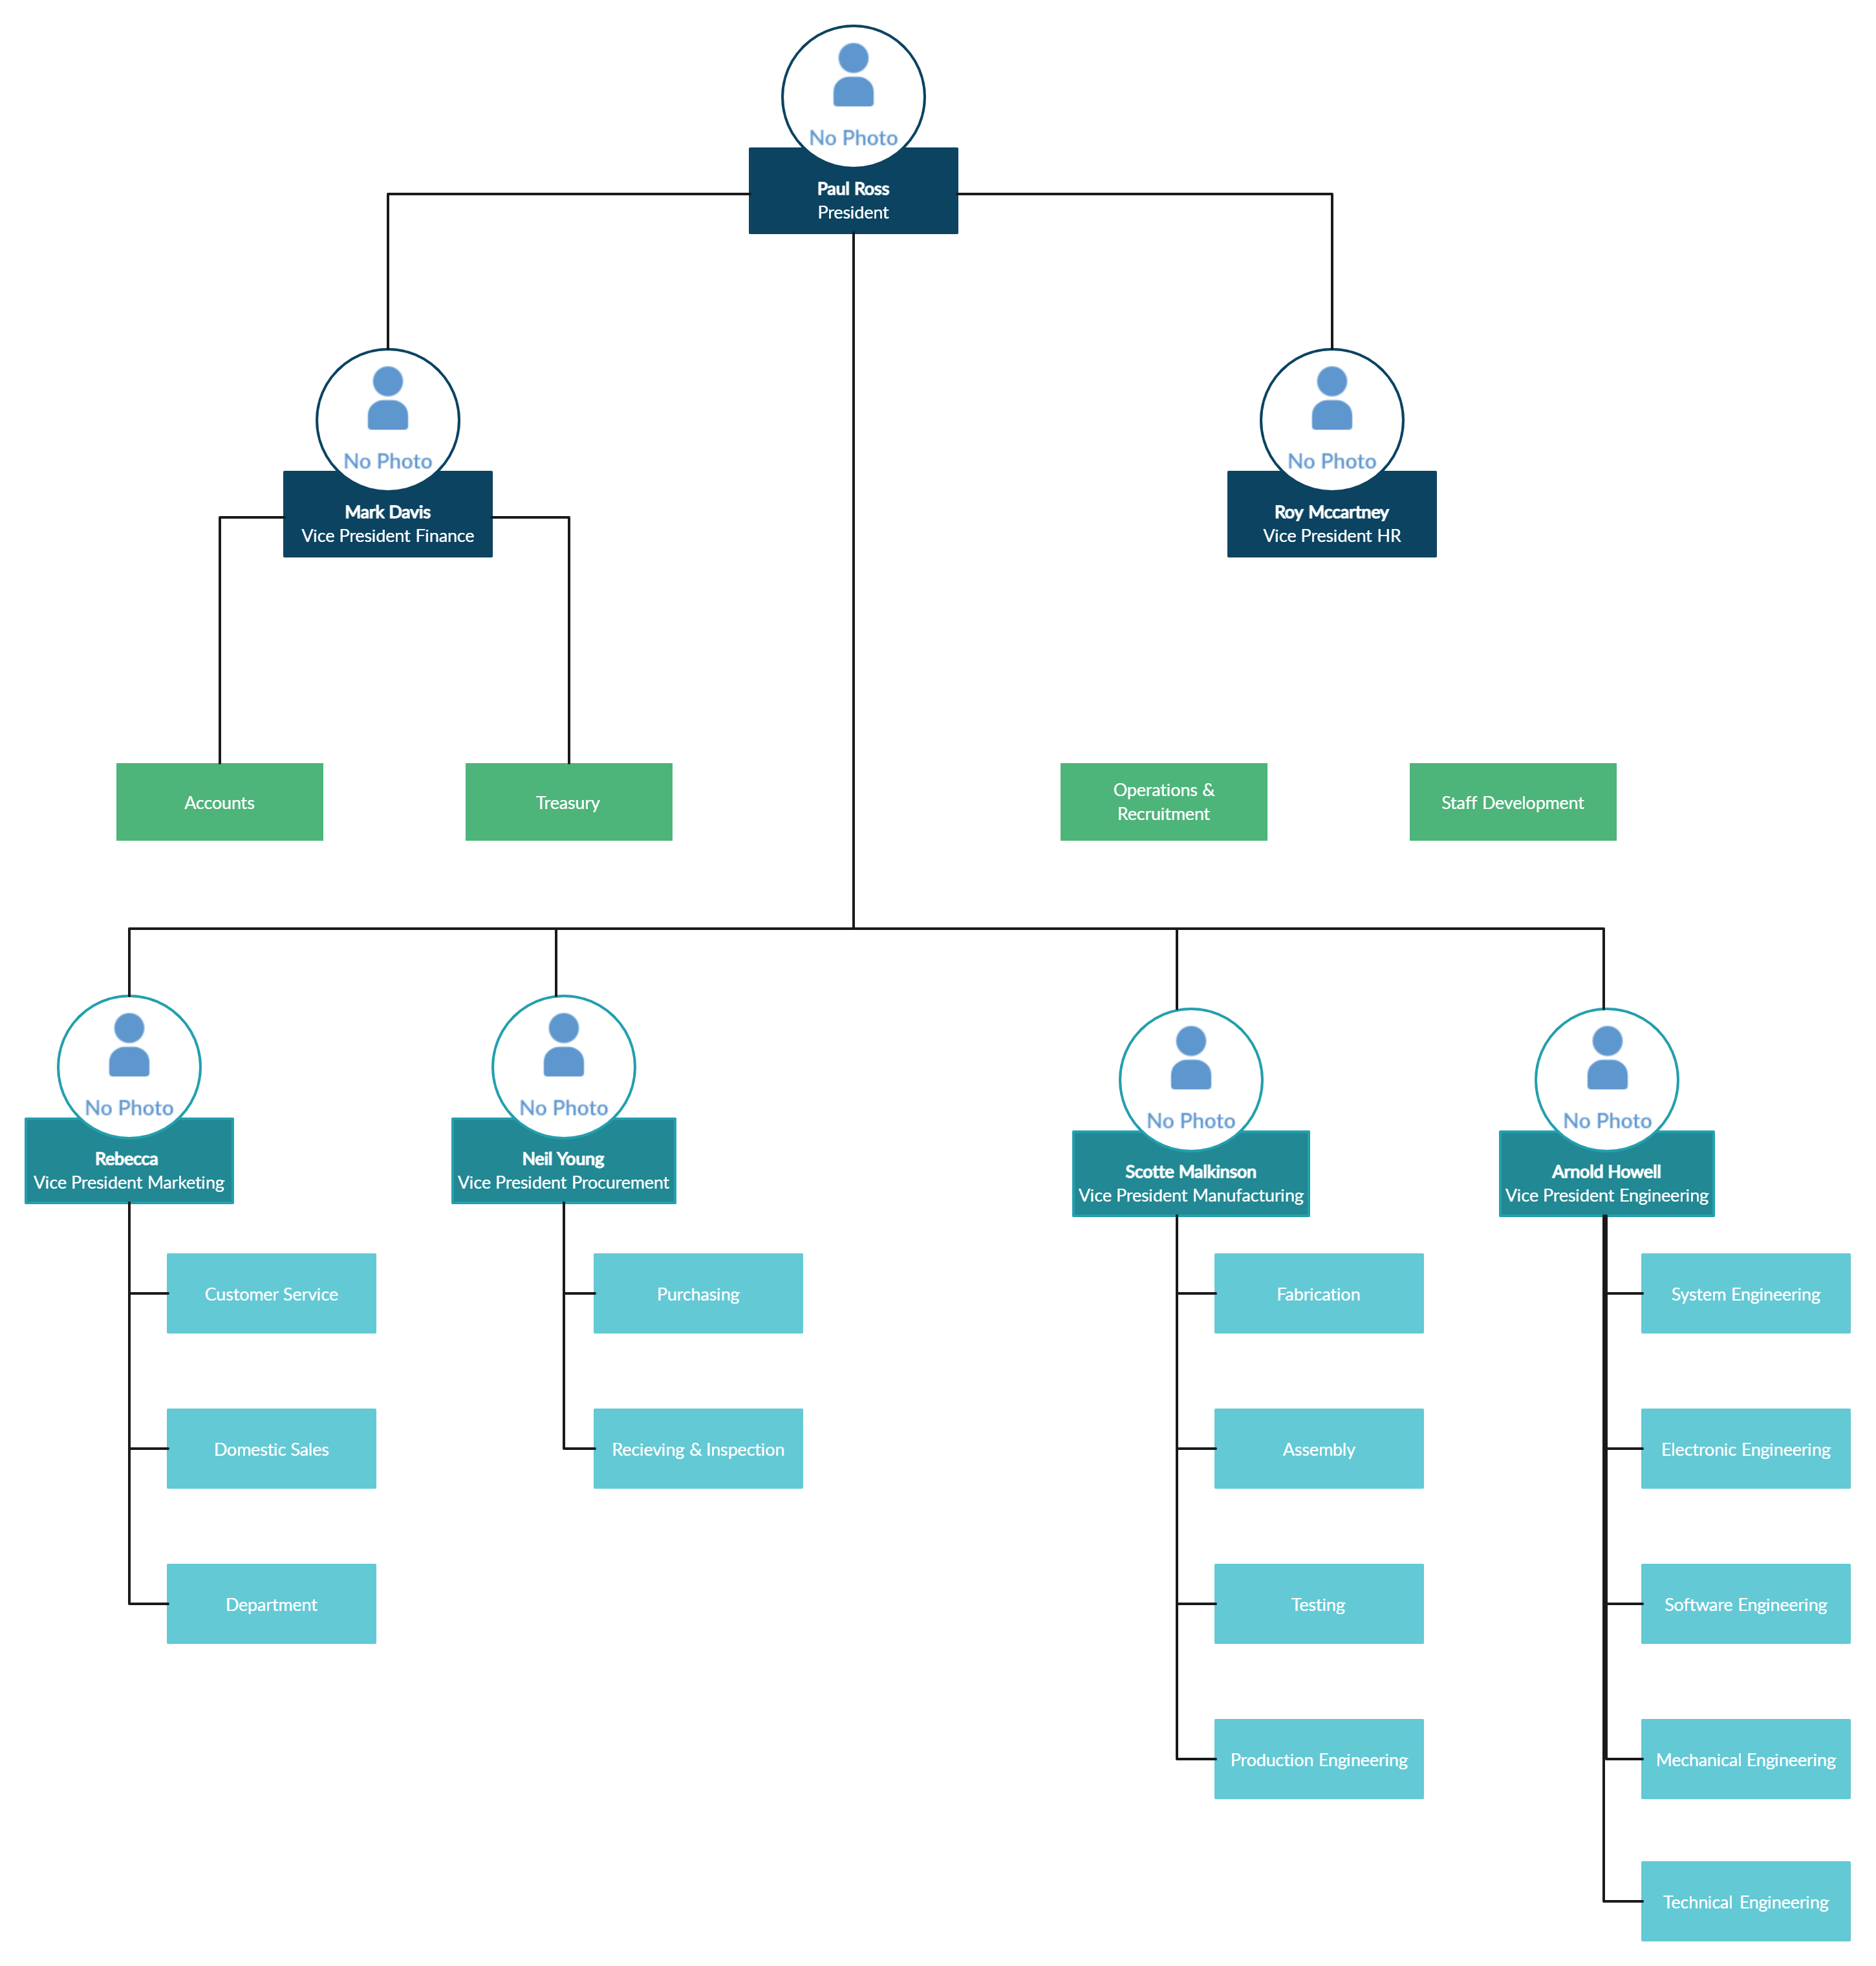
\includegraphics[width=12cm]{Figures/Organizational_Chart.png}
    \caption{Organizational Chart}
    %\label{fig:my_label} %Optional (If you want to reference the figure in later chapters)
\end{figure}











\section{Presentation of the project}


\subsection{Project Framework}



\subsection{Project objectives}





\subsection{Project Planning}

\begin{figure}[H] 
    \centering
    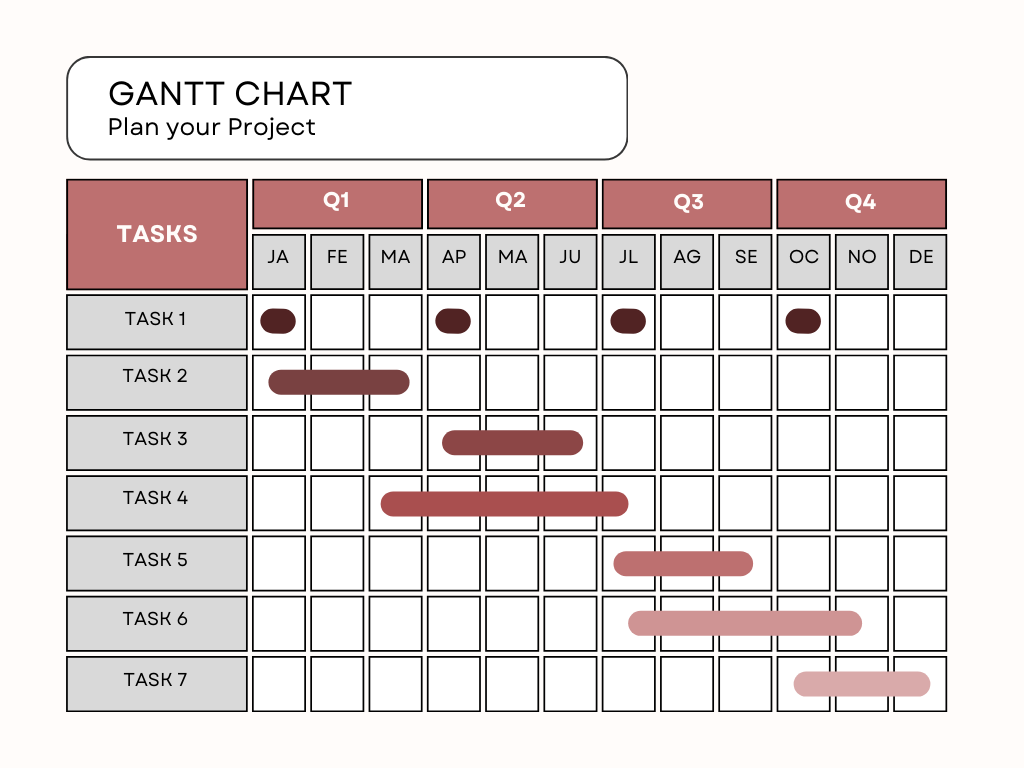
\includegraphics[width=12cm]{Figures/Gantt_Diagram.png}
    \caption{Gantt Diagram}
    %\label{fig:my_label} %Optional (If you want to reference the figure in later chapters)
\end{figure}

\newpage

\section*{Conclusion}

Lorem ipsum dolor sit amet, consectetur adipiscing elit. Praesent nec dapibus justo. Donec sagittis vulputate ante sed porttitor. Suspendisse sit amet nisl massa. Curabitur nec nisl condimentum, egestas ex vitae, dapibus enim. Etiam iaculis, erat faucibus pellentesque sagittis, nisi justo sollicitudin nibh, et condimentum augue massa non turpis. Proin commodo enim fermentum suscipit condimentum. Maecenas molestie, dui nec vestibulum rhoncus, arcu nisl faucibus neque, a ornare nisi massa ac eros. Aenean id velit sit amet lacus mattis varius. Donec fringilla massa sed nisi eleifend, a aliquet mi tempus. Nunc posuere euismod est, nec tristique augue lobortis non. Sed sodales sem ut metus tempus ullamcorper.
